%%%%%%%%%%%%%%%%%%%%%%%%%%%%%%%%%%%%%%%%%
% Daily Laboratory Book
% LaTeX Template
%
% This template has been downloaded from:
% http://www.latextemplates.com
%
% Original author:
% Frank Kuster (http://www.ctan.org/tex-archive/macros/latex/contrib/labbook/)
%
% Important note:
% This template requires the labbook.cls file to be in the same directory as the
% .tex file. The labbook.cls file provides the necessary structure to create the
% lab book.
%
% The \lipsum[#] commands throughout this template generate dummy text
% to fill the template out. These commands should all be removed when 
% writing lab book content.
%
% HOW TO USE THIS TEMPLATE 
% Each day in the lab consists of three main things:
%
% 1. LABDAY: The first thing to put is the \labday{} command with a date in 
% curly brackets, this will make a new page and put the date in big letters 
% at the top.
%
% 2. EXPERIMENT: Next you need to specify what experiment(s) you are 
% working on with an \experiment{} command with the experiment shorthand 
% in the curly brackets. The experiment shorthand is defined in the 
% 'DEFINITION OF EXPERIMENTS' section below, this means you can 
% say \experiment{pcr} and the actual text written to the PDF will be what 
% you set the 'pcr' experiment to be. If the experiment is a one off, you can 
% just write it in the bracket without creating a shorthand. Note: if you don't 
% want to have an experiment, just leave this out and it won't be printed.
%
% 3. CONTENT: Following the experiment is the content, i.e. what progress 
% you made on the experiment that day.
%
%%%%%%%%%%%%%%%%%%%%%%%%%%%%%%%%%%%%%%%%%

%----------------------------------------------------------------------------------------
%	PACKAGES AND OTHER DOCUMENT CONFIGURATIONS
%----------------------------------------------------------------------------------------

\documentclass[idxtotoc,hyperref,openany]{labbook} % 'openany' here removes the gap page between days, erase it to restore this gap; 'oneside' can also be added to remove the shift that odd pages have to the right for easier reading

\usepackage[ 
  backref=page,
  pdfpagelabels=true,
  plainpages=false,
  colorlinks=true,
  bookmarks=true,
  pdfview=FitB]{hyperref} % Required for the hyperlinks within the PDF
  
\usepackage{booktabs} % Required for the top and bottom rules in the table
\usepackage{float} % Required for specifying the exact location of a figure or table
\usepackage{graphicx} % Required for including images
\usepackage{lipsum} % Used for inserting dummy 'Lorem ipsum' text into the template
\usepackage{xeCJK}
\usepackage{hyperref}
%\usepackage{color}
\usepackage[usenames, dvipsnames]{color}
\definecolor{mygray}{gray}{0.8}
%\setCJKmainfont{DFMing-Md-HK-BF.ttf}
\setCJKmainfont{wqy-microhei.ttc}
\newcommand{\HRule}{\rule{\linewidth}{0.5mm}} % Command to make the lines in the title page
\setlength\parindent{0pt} % Removes all indentation from paragraphs

%----------------------------------------------------------------------------------------
%	DEFINITION OF EXPERIMENTS
%----------------------------------------------------------------------------------------

\newexperiment{example}{This is an example experiment}
\newexperiment{example2}{This is another example experiment}
\newexperiment{example3}{This is yet another example experiment}
\newexperiment{table}{This shows a sample table}
%\newexperiment{shorthand}{Description of the experiment}

%---------------------------------------------------------------------------------------

\begin{document}

%----------------------------------------------------------------------------------------
%	TITLE PAGE
%----------------------------------------------------------------------------------------

\frontmatter % Use Roman numerals for page numbers
\title{
\begin{center}
\HRule \\[0.4cm]
{\Huge \bfseries Laboratory Journal \\[0.5cm] \Large Master of Science}\\[0.4cm] % Degree
\HRule \\[1.5cm]
\end{center}
}
\author{\Huge 梁家萁 \\ \\ \LARGE jcliang@cycu.org.tw \\[2cm]} % Your name and email address
\date{Beginning 6 February 2012} % Beginning date
\maketitle

\tableofcontents

\mainmatter % Use Arabic numerals for page numbers

%----------------------------------------------------------------------------------------
%	LAB BOOK CONTENTS
%----------------------------------------------------------------------------------------

% Blank template to use for new days:

%\labday{Day, Date Month Year}

%\experiment{}

%Text

%-----------------------------------------

%\experiment{}

%Text

%----------------------------------------------------------------------------------------

\labday{Friday, 25 November 2011}

\experiment{example}

\lipsum[1]

%-----------------------------------------

\experiment{example2} % Multiple experiments can be included in a single day, this allows you to segment what was done each day into separate categories

\begin{figure}[H] % Example of including images
\begin{center}

\includegraphics[width=0.5\linewidth]{example_figure}
\end{center}
\caption{Example figure.}
\label{fig:example_figure}
\end{figure}

%-----------------------------------------

\experiment{example3}

\lipsum[3-5]

%----------------------------------------------------------------------------------------

\labday{Friday, 26 March 2010}

\experiment{table}

\begin{table}[H]
\begin{tabular}{l l l}
\toprule
\textbf{Groups} & \textbf{Treatment X} & \textbf{Treatment Y} \\
\toprule
1 & 0.2 & 0.8\\
2 & 0.17 & 0.7\\
3 & 0.24 & 0.75\\
4 & 0.68 & 0.3\\
\bottomrule
\end{tabular}
\caption{The effects of treatments X and Y on the four groups studied.}
\label{tab:treatments_xy}
\end{table}

Table \ref{tab:treatments_xy} shows that groups 1-3 reacted similarly to the two treatments but group 4 showed a reversed reaction.

%----------------------------------------------------------------------------------------

\labday{Saturday, 27 March 2010}

\experiment{Bulleted list example} % You don't need to make a \newexperiment if you only plan on referencing it once

This is a bulleted list:

\begin{itemize}
\item Item 1
\item Item 2
\item \ldots and so on
\end{itemize}

%-----------------------------------------

\experiment{example}

\lipsum[6]

%-----------------------------------------

\experiment{example2}

\lipsum[7]
%-----------------------------------------

%----------------------------------------------------------------------------------------
%	FORMULAE AND MEDIA RECIPES
%----------------------------------------------------------------------------------------

\labday{} % We don't want a date here so we make the labday blank

\begin{center}
\HRule \\[0.4cm]
{\huge \textbf{Formulae and Media Recipes}}\\[0.4cm] % Heading
\HRule \\[1.5cm]
\end{center}

%----------------------------------------------------------------------------------------
%	MEDIA RECIPES
%----------------------------------------------------------------------------------------

\newpage

\huge \textbf{Media} \\ \\

\normalsize \textbf{Media 1}\\
\begin{table}[H]
\begin{tabular}{l l l}
\toprule
\textbf{Compound} & \textbf{1L} & \textbf{0.5L}\\
\toprule
Compound 1 & 10g & 5g\\
Compound 2 & 20g & 10g\\
\bottomrule
\end{tabular}
\caption{Ingredients in Media 1.}
\label{tab:med1}
\end{table}

%-----------------------------------------

%\textbf{Media 2}\\ \\

%Description

%----------------------------------------------------------------------------------------
%	FORMULAE
%----------------------------------------------------------------------------------------

\newpage

\huge \textbf{Formulae} \\ \\

\normalsize \textbf{Formula 1 - Pythagorean theorem}\\ \\
$a^2 + b^2 = c^2$\\ \\

%-----------------------------------------

%\textbf{Formula X - Description}\\ \\

%Formula

%----------------------------------------------------------------------------------------
\labday{Wednesday, 27 September 2017}

\experiment{編號.實驗名稱}


\begin{enumerate}
\item 問題原因:

會發生這個問題是因為......


\item 解決辦法:

我用這樣這樣那樣那樣解決者個問題
	\begin{itemize}
	\item 第一步驟
	
	\colorbox{mygray}{\$ cmd指令1}
	
	\item 第二步驟
	
	\colorbox{mygray}{\$ cmd指令2}
	
	\item 第三步驟
		
	\colorbox{mygray}{\$ cmd指令3}
	
	\end{itemize}
\end{enumerate}

\experiment{編號.實驗名稱}


\begin{enumerate}
	\item 問題原因:
	
	會發生這個問題是因為......
	
	
	\item 解決辦法:
	
	我用這樣這樣那樣那樣解決者個問題
	\begin{itemize}
		\item 第一步驟
		
		\colorbox{mygray}{\$ cmd指令1}
		
		\item 第二步驟
		
		\colorbox{mygray}{\$ cmd指令2}
		
		\item 第三步驟
		
		\colorbox{mygray}{\$ cmd指令3}
		
	\end{itemize}
\end{enumerate}







\labday{Wednesday, 27 September 2017}

\experiment{解決每次重新開啟終端機,需要重新設定\$GOPATH的問題。}


\begin{enumerate}
\item 問題原因

因為使用gvm作為go語言的版本控管器,選擇go版本後,會去抓g01.9這個檔案,裡面的環境變數是gvm預設的,所以每次都要重新設定。

\item 解決辦法

自訂一個環境變數,選擇go版本之後,指定環境變數檔。
	\begin{itemize}
	\item 選擇go版本,我選擇go1.9
	
	\colorbox{mygray}{\$ gvm use go1.9}

	\item 在此版本下加入自訂環境變數”test”
	
	\colorbox{mygray}{\$ gvm pkgset create test}
	\item 進到此資料夾「~./gvm/environments/」,找到「go1.9@test.txt」檔。修改此檔案,在檔案最後面加上以下兩行。
	
	\colorbox{mygray}{export GOPATH=”/home/user/goroot”}
	
	\colorbox{mygray}{export PATH=”\$GOPATH/bin:\$PATH”}
	\item 在終端機下指令,指定使用test環境變數
	
	\colorbox{mygray}{\$ gvm pkgset use test}
	\end{itemize}
\end{enumerate}


\labday{Friday, 29 September 2017}

\experiment{執行bee run時,網頁無法正常運行,出現 ListenAndServe:  listen tcp :8080: bind: address already in use。}


\begin{enumerate}
\item 問題原因:

因為在github上的程式碼有問題。當初直接複製test資料夾裡的hello資料夾,main.go以及routets.go的程式碼,import的pakage路徑都還是test/hello/…...>,所以出現錯誤。按下ctrl+C後,並沒有正常的關閉server,所以改完程式碼,執行bee run時,會顯示port以被監聽。


\item 解決辦法:

用指令強置殺掉port:8080

	\begin{itemize}
	\item 
	\colorbox{mygray}{\$ lsof -ti:8080 |xargs kill -9}
	
	\item 結果chrome直接被我關掉,連其他瀏覽終的網頁都關了。
	
	
	\end{itemize}
\end{enumerate}





\labday{Monday, 15 January 2018}

\experiment{製作git與goroot工作環境的連結}


\begin{enumerate}
\item 問題原因:

git抓下來的資料夾除了go語言程式碼之外,還有其他資料,都放到goroot裡面很雜亂。然而,go語言的程式碼只能在goroot的工作還行下執行,所以要製作連結,把程式碼連到goroot裡。

\item 解決辦法:

將git的檔案連結到goroot,goroot裡只放要執行的程式碼。
	\begin{itemize}
	\item 進到go語言執行環境資料夾
	
	\colorbox{mygray}{\$ code goroog/src/jyw}
	
	\item 使用指令ln -s <git-folder> \colorbox{yellow}{{\color{blue}<link-name>}}建立連結資料夾。
	
	{\color{blue}<link-name>:goroot裡連結資料夾的名字}
	
	\colorbox{mygray}{\$ ln -s /home/liang/class-learning/go \colorbox{yellow}{class-learning}}
	
	\item 此時jyw目錄下會增加一個「class-learning」連結資料夾,在此修改的內容會同步到git的資料夾。
			
	\end{itemize}
\end{enumerate}

\experiment{建立「RefVer」(reference version)標籤}


\begin{enumerate}
	\item 問題原因:
	
	因為要將老師之前寫的網頁蓋掉,所以先建立一個git的標籤(tag),之後需要參考時,checkout 此標籤即可。	
	
	\item 解決辦法:
	
	建立「RefVer」標籤
	\begin{itemize}
		\item 第一步驟
		
		\colorbox{mygray}{\$ git tag RefVer
			}
		
		\item 第二步驟
		
		\colorbox{mygray}{\$ git push origin RefVer}
			
	\end{itemize}
\end{enumerate}

%\experiment{製作layout.tpl}
\experiment{製作layout.tpl}

\begin{enumerate}
	\item 問題原因:
	
	每個頁面都有相同的header以及footer,製作layout.tpl樣板,可以讓每個頁面的頭尾都相同。	
	
	\item 解決辦法:
	
	\begin{itemize}
		\item 將sample.html貼到layout.tpl檔,body的部份用\{\{.LayoutContent\}\}取代。
				
		\item 修改layout.tpl中css、js、fonts…...等的路徑,改成/static/css/…….。
		
		\item 將bootstrap的css、js、fonts…...等的檔案,複製到static下對應的路徑。
		
		\item 將homepage.html中body的部份貼到index.tpl裡。
		
		\item 其他細節參考米聽紀錄106/09/29
		
		\url{https://drive.google.com/open?id=1nxYJ4HLNCTJvEDQu7bVTM1Fs-pM4SiKjOUr1xN55fYg}
		
	\end{itemize}
\end{enumerate}





\labday{Tuesday, 16 January 2018}

\experiment{修改layout,在nav-bar加上setting-icon}


\begin{enumerate}
\item 問題原因:


\item 解決辦法:

修改bootstrap studio中smaple.html的檔案,重新匯出。
	
\end{enumerate}


\experiment{在bootstrap studio中,做link components。}


\begin{enumerate}
	\item 問題原因:
	
	將所有頁面的header以及footer都連結到sample.html,無論在哪個頁面修改頭尾,所有頁面的html都會跟著改。	
	
	\item 解決辦法:
	
	參考此網頁
	\url{https://bootstrapstudio.io/forums/topic/linked-components/}
	\begin{itemize}
		\item 選擇要複製的元件,右鍵→Copy。
			
		\item 到其他頁面,右鍵→Paste Linked。
		
		\colorbox{yellow}{※在其他頁面時,對著右上角option的block按右鍵。}
			
		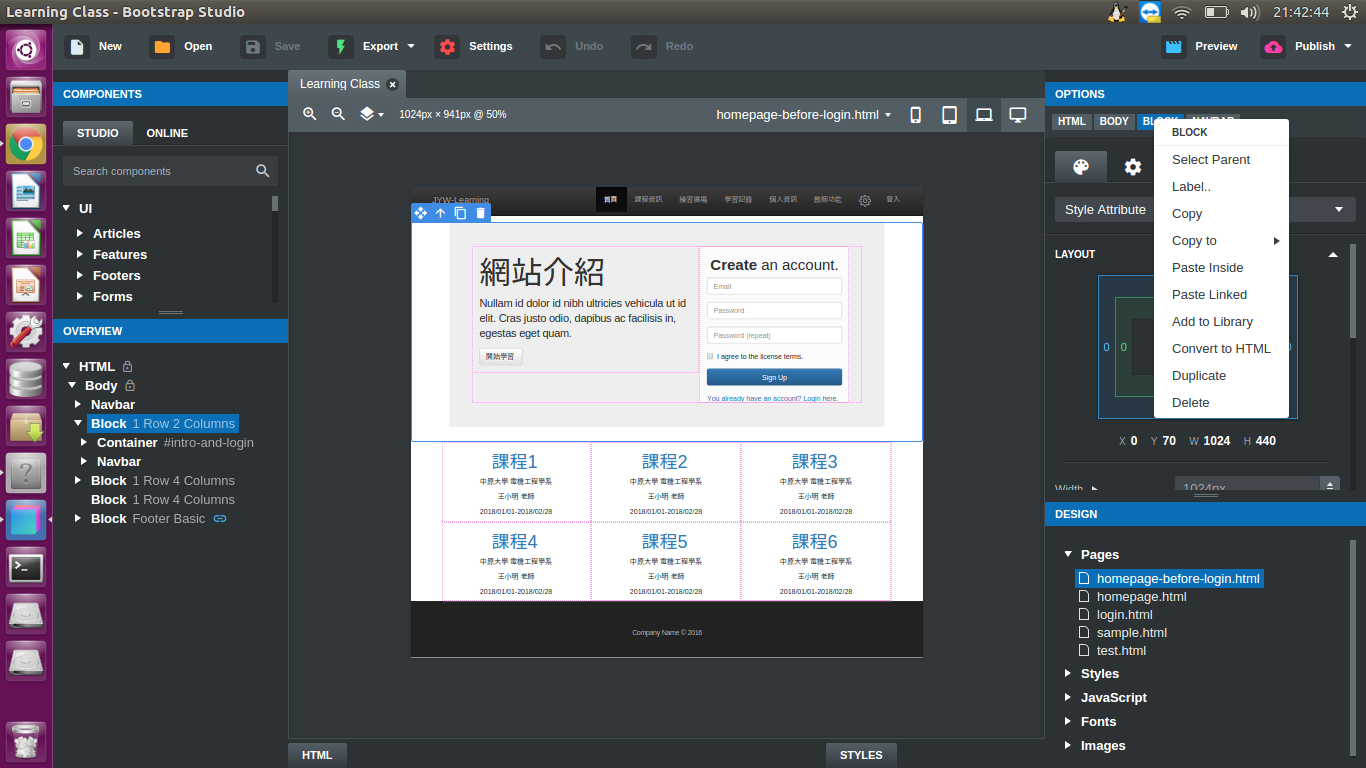
\includegraphics[width=0.8\textwidth]{fig/fig01}
		\item homepage-before-login沒有link nav-bar
	\end{itemize}
\end{enumerate}







\end{document}